\section{Random Number Generators}
\label{section:RNGs}

% This section was authored by Ralf Schlatterbeck (Ralf Schlatterbeck <rsc@runtux.com>)

\epigraph{``The generation of random numbers is too important to be left to chance.''}{Robert R. Coveyou}


\begin{figure}[h]
  \centering
  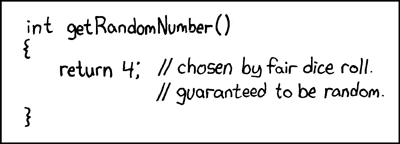
\includegraphics[width=0.4\textwidth]{img/random_number.png}
  \caption{xkcd, source: \url{https://imgs.xkcd.com/comics/random_number.png}, license: CC-BY-NC}
  \label{fig:dilbertRNG}
\end{figure}



A good source of random numbers is essential for many crypto
operations. The key feature of a good random number generator is the
non-predictability of the generated numbers. This means that hardware
support for generating entropy is essential.


Hardware random number generators in operating systems or standalone
components collect entropy from various random events mostly by using
the (low bits of the) time an event occurs as an entropy source. The
entropy is merged into an entropy pool and in some implementations there
is some bookkeeping about the number of random bits available.

\subsection{When random number generators fail}

Random number generators can fail -- returning predictable non-random
numbers -- if not enough entropy is available when random numbers should
be generated.

This typically occurs for embedded devices and virtual machines.
Embedded devices lack some entropy sources other devices have, e.g.:

\begin{itemize*}
  \item No persistent clock, so boot-time is not contributing to the
    initial RNG state
  \item No hard-disk: No entropy from hard-disk timing, no way to store
    entropy between reboots
\end{itemize*}

Virtual machines emulate some hardware components so that the
generated entropy is over-estimated. The most critical component that
has been shown to return wrong results in an emulated environment is the
timing source~\cite{Eng11,POL11}.

Typically the most vulnerable time where low-entropy situations occur is
shortly after a reboot. Unfortunately many operating system installers
create cryptographic keys shortly after a reboot~\cite{HDWH12}.

Another problem is that OpenSSL seeds its internal random generator only
seldomly from the hardware random number generator of the operating
system. This can lead to situations where a daemon that is started at a
time when entropy is low keeps this low-entropy situation for hours
leading to predictable session keys~\cite{HDWH12}.

\subsection{Linux}
\label{subsec:RNG-linux}

\todo{Other architectures, BSD, Windows?}

On Linux there are two devices that return random bytes when read; the
\verb+/dev/random+ can block until sufficient entropy has been collected
while \verb+/dev/urandom+ will not block and return whatever (possibly
insufficient) entropy has been collected so far.

Unfortunately most crypto implementations are using \verb+/dev/urandom+
and can produce predictable random numbers if not enough entropy has
been collected~\cite{HDWH12}.

Linux supports the injection of additional entropy into the entropy pool
via the device \verb+/dev/random+. On the one hand this is used for
keeping entropy across reboots by storing output of /dev/random into a
file before shutdown and re-injecting the contents during the boot
process. On the other hand this can be used for running a secondary
entropy collector to inject entropy into the kernel entropy pool.

On Linux you can check how much entropy is available with the command:
\begin{lstlisting}
$ cat /proc/sys/kernel/random/entropy_avail
\end{lstlisting}

%% specifics for libraries
%% Openssl uses /dev/urandom. See the paper: https://factorable.net/weakkeys12.conference.pdf (section 5.2)
%% What about other libs? 
%% What about other OSes? 


\subsection{Recommendations}

To avoid situations where a newly deployed server doesn't have enough
entropy it is recommended to generate keys (e.g. for SSL or SSH) on
a system with a sufficient amount of entropy available and transfer the generated keys
to the server.  This is especially advisable for small embedded devices
or virtual machines.

For embedded devices and virtual machines deploying additional userspace
software that generates entropy and feeds this to kernel entropy pool
(e.g. by writing to \verb+/dev/random+ on Linux) is recommended. Note
that only a process with root rights can update the entropy counters in the
kernel; non-root or user processes can still feed entropy to the pool but
cannot update the counters~\cite{Wikipedia:/dev/random}.

For Linux the \verb+haveged+
implementation~\cite{HAV13a} based on the HAVEGE~\cite{SS03}
strong random number generator currently looks like the best choice. It
can feed its generated entropy into the kernel entropy pool and recently
has grown a mechanism to monitor the quality of generated random
numbers~\cite{HAV13b}. The memory footprint may be too high for small
embedded devices, though.

For systems where -- during the lifetime of the keys -- it is expected
that low-entropy situations occur, RSA keys should be preferred over DSA
keys: For DSA, if there is ever insufficient entropy at the time keys
are used for signing this may lead to repeated ephemeral keys. An
attacker who can guess an ephemeral private key used in such a signature
can compromise the DSA secret key.
For RSA this can lead to discovery of encrypted plaintext or forged
signatures but not to the compromise of the secret key~\cite{HDWH12}.
